\documentclass[12pt]{extarticle}
\usepackage{tempora}
\usepackage[T1, T2A]{fontenc}
\usepackage[utf8]{inputenc}
\usepackage[english, ukrainian]{babel}
\usepackage{geometry}
\usepackage{graphicx}
\usepackage{multirow}
\usepackage{multicol}
\usepackage{float}
\graphicspath{{/home/artem/Pictures}}
\geometry
{
    a4paper,
    left=30mm,
    top=15mm,
    right=20mm,
    bottom=15mm,
}

\begin{document}
\begin{titlepage}
    \begin{center}
        \textbf{\normalsize{\MakeUppercase{
            Міністерство Освіти і науки України
            Національний університет "Львівська політехніка"
        }}}

        \begin{flushright}
        \textbf{ІКНІ}\\
        Кафедра \textbf{ПЗ}
        \end{flushright}
        \vspace{15mm}

        \includegraphics[width=0.4\textwidth]{lpnu_logo.png}

        \vspace*{\fill}

        \textbf{\normalsize{\MakeUppercase{Звіт}}}
            
        До лабораторної роботи №7

        \textbf{на тему:} “Статичні та динамічні бібліотеки. WINDOWS та LINUX”

        \textbf{з дисципліни:} “Операційні системи”
            
        \vspace*{\fill}

        \begin{flushright}

            \textbf{Лектор:}\\
            старший викладач кафедри ПЗ\\
            Грицай О.Д.\\
            \vspace{12pt}

            \textbf{Виконав:}\\
            студент групи ПЗ-24\\
            Губик А. С.\\
            \vspace{12pt}

            \textbf{Прийняв:}\\
            доцент кафедри ПЗ\\
            Горечко О. М.\\
        \vspace{12pt}
        \end{flushright}

        Львів -- 2023
            
            
    \end{center}
\end{titlepage}

\textbf{Тема роботи:}Статичні та динамічні бібліотеки. WINDOWS та LINUX
\vspace{12pt}

\textbf{Мета роботи:}Ознайомитися з статичними та динамічними бібліотеками в операційних
системах WINDOWS та LINUX. Навчитися реалізовувати статичні та динамічні
бібліотеки.

\subsection*{Теоретичні відомості}
Створення програмного забезпечення довгий і дорогий процес, тому існує
необхідність його спростити та оптимізувати для подальшого модифікування
застосунків. Часто виникає необхідність використання одних і тих ж функцій або
даних у різних частинах проекту. Частина функцій у проекті використовується
рідко, а частина при створені нової версії застосунку буде постійно змінюватись
або додаватимуться нові функції. Крім того, всі дані можна розділити за певною
тематикою або за видом ресурсів і т.д. Також потрібно передбачити оновлення
даних. Тому виникає необхідність винести частину коду і даних з основної
частин проекту в окремі приєднанні модулі.
Зрозуміло, що виносити кожну функцію або екземпляр даних в окремий
файл чи модуль недоцільно, оскільки це спричинить довший відгук від
програмного продукту, навантажить систему додатковими викликами, що у свою
чергу зменшить продуктивність і ефективність застосунку. Зазвичай функції або
дані об’єднують згідно функціональності, за тематикою та іншими
властивостями в окремі скомпільовані спеціальні об’єктні файли – бібліотеки.
Бібліотека – це файл, що містить один або декілька об’єктних файлів для
вирішення близьких за тематикою завдань у розробці програмних продуктів. У
бібліотеці можуть міститися об’єктні модулі, програмний код або дані, що
можуть використовуватись окремо або разом на різних етапах створення проекту
(компілювання, лінкування, завантаження чи виконання).
Бібліотека містить символьний індекс, який складається з назв функцій і
змінних, які містяться у бібліотеці. Це дозволяє прискорити процес лінкування
програми, оскільки пошук функцій і змінних в об'єктних файлах бібліотеки
відбувається набагато швидше, ніж пошук в наборі вказаних об'єктних файлів.
Тому використання бібліотеки дозволяє компактно зберігати усі необхідні
об'єктні файли в одному місці, і при цьому значно підвищити швидкість
компіляції.
Бібліотеки прийнято розділяти відповідно до способу з’єднання на
статичні та динамічні. Статичні бібліотеки зв’язуються з проектом перед
завантаженням і є частиною бінарного файлу. Динамічні можуть бути зв’язані з
проектом статично і динамічно. У різних операційних системах є свої
особливості створення і використання бібліотек

\subsection*{Linux}


\begin{figure}[H]
    \centering
    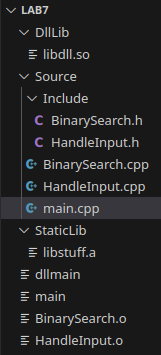
\includegraphics[width=0.60\textwidth]{dir}
    \caption{Вміст директорій}
\end{figure}

\begin{figure}[H]
    \centering
    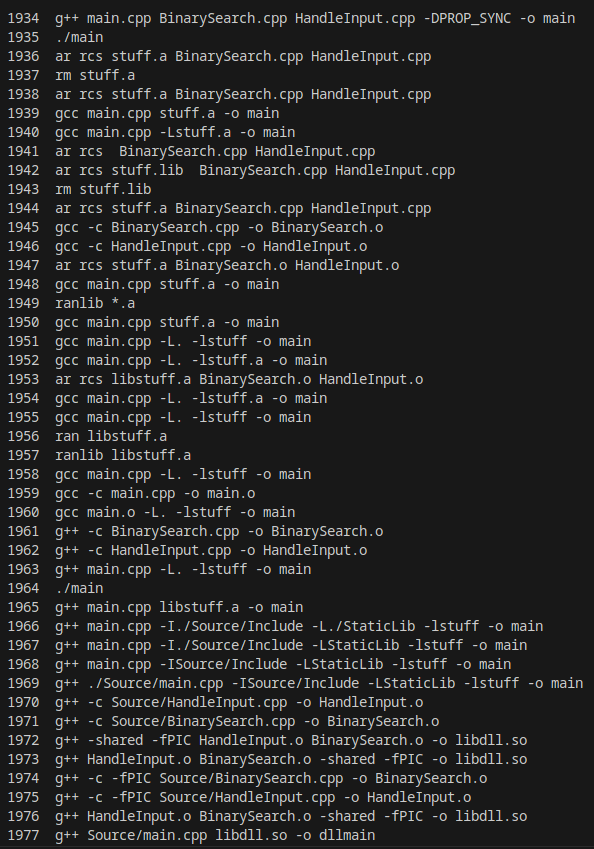
\includegraphics[width=0.90\textwidth]{console}
    \caption{Використані команди}
\end{figure}

\subsection*{Windows}

\begin{figure}[H]
    \centering
    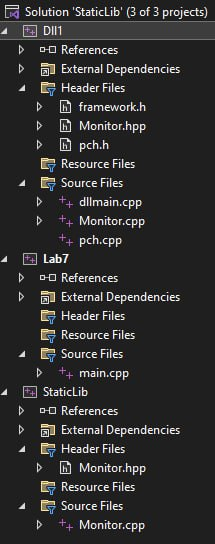
\includegraphics[width=0.60\textwidth]{lfolder}
    \caption{Вміст директорій}
\end{figure}

\begin{figure}[H]
    \centering
    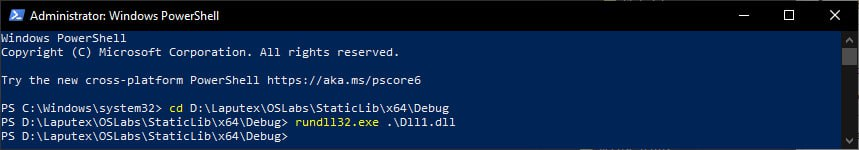
\includegraphics[width=0.99\textwidth]{cmd}
    \caption{}
\end{figure}

\textbf{Висновок:}
Я навчився створюваи динамічні та статичні бібліотеки на Linux i Windows.
 \end{document}
